\begin{frame}{Power Analysis Attacks}

\begin{itemize}
\item Power consumption during the execution of programs depends on intermediate values.
\pause
\item Power analysis attacks leverage this fact to find the secret key. 
\pause
\end{itemize}
\vspace{-4pt}
\begin{figure}
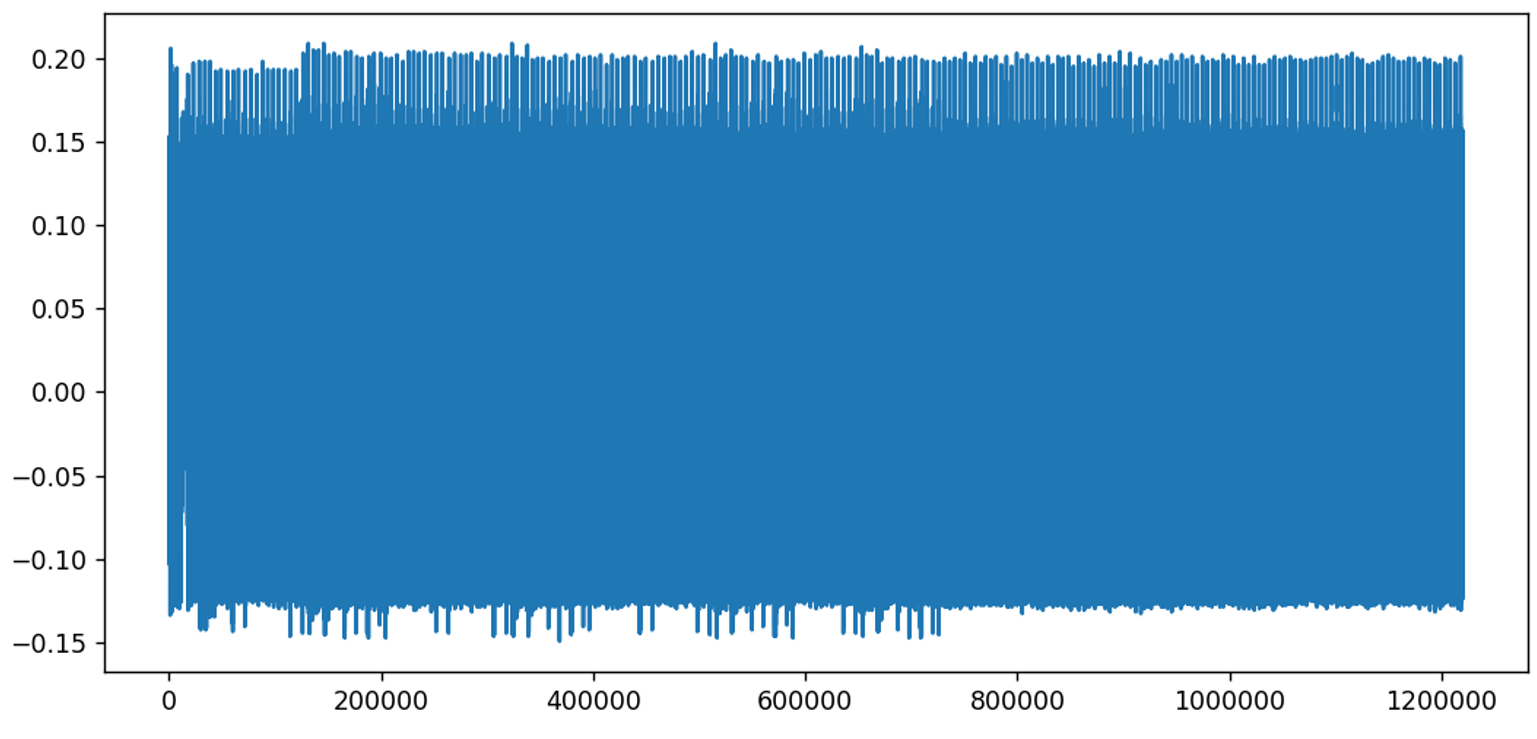
\includegraphics[width=.7\textwidth]{Figure/trace_example_ECC.png}
\vspace{-5pt}
\caption{An Example of a Power Trace}
\end{figure}

\end{frame}



\begin{frame}{Masking}

Masking defends against such threats by secret-sharing the sensitive variables.
\pause
\begin{itemize}
	\item Boolean Masking: A variable $x$ is split into $n$ shares $(x_i)_{1 \leq i \leq n}$ such that
	\[
	x = \bigoplus_{i=1}^n x_i
	\]
	\pause
	\item Arithmetic Masking: A variable $x$ is split into $n$ shares $(x_i)_{1 \leq i \leq n}$ (when stored in a $k$-bit register) such that
	\[
	x = \sum_{i=1}^n x_i \quad (\bmod\; 2^k)
	\]
\end{itemize}

\end{frame}


\begin{frame}{Masking}

\begin{itemize}
\item In each run, all $x_i$'s are randomized so that any $n-1$ shares of them are independently and uniformly distributed.
\pause
\item All operations need to be operated via shares.
\end{itemize}
\pause
For example, if $x$ is a secret variable, the operation $y \gets {\sf pt} \oplus x$ will become 
\[
	\begin{cases} y_1 \gets {\sf pt} \oplus x_1 \\ y_2 \gets x_2  \end{cases} \text{where } x_1,x_2 \getsdollar \{0,1\}^*, x_1 \oplus x_2 = x
\]

The variables with secret information are splitted into shares.

\end{frame}


%\begin{frame}{Probing Model}
%
%\begin{itemize}
%	\item The $t$-probing model \cite{C:IshSahWag03} assumes that an adversary is able to peek any $t$ intermediate values in the algorithm.
%	\item To be secure in $t$-probing model, $n \geq t+1$, and any share cannot be combined with each other.
%	\item It is complicated to prove $t$-probing security for a large composition of small algorithms (gadget). The concept of non-interference is convenient in this case.
%\end{itemize}
%
%\end{frame}
%
%
%
%\begin{frame}{Non-Interference Security}
%
%\begin{definition}{$t$-Non-Interference ($t$-NI) Security (from \cite{CCS:BBDFGS16})}
%A gadget is $t$-Non-Interference ($t$-NI) secure if every set of $t$ intermediate values can be simulated by no more than $t$ shares of each of its inputs.
%\end{definition}
%\medskip
%
%\begin{definition}{$t$-Strong Non-Interference ($t$-SNI) Security (from \cite{CCS:BBDFGS16})}
%A gadget is $t$-Strong-Non-Interference ($t$-SNI) secure if for every set of $t_I$ internal intermediate values and $t_O$ of its output shares with $t_I + t_O \leq t$, they can be simulated by no more than $t_I$ shares of each of its inputs.
%\end{definition}
%\medskip
%
%\end{frame}
%
%
%\begin{frame}{Non-Interference Security}
%
%In a nutshell,
%\begin{itemize}
%	\item $t$-SNI is stronger than $t$-NI by definition.
%	\item If a gadget is $t$-NI secure, and if any $n-1$ input shares are uniformly and independently distributed, then it is $t$-probing secure.
%	\item A composition of $t$-NI gadgets may not be $t$-NI, so we insert $t$-SNI gadgets to make it $t$-NI or $t$-SNI.
%\end{itemize}
%
%\end{frame}
